\documentclass[12pt, letterpaper]{article}
\usepackage[utf8]{inputenc}
\usepackage[left = 2.5cm, right = 2.5cm, top = 2.5cm, bottom = 2.5cm]{geometry}
\usepackage{amsthm}
\usepackage{amsfonts}
\usepackage{amsmath}
\usepackage{amssymb}
\usepackage{graphicx}
\usepackage[T1]{fontenc}

\author{Hernández Ferreiro Enrique Ehecatl \\
        López Soto Ramses Antonio \\
        Miguel Torres Eric Giovanni \\
        Quintero Villeda Erik}

\title{Tarea 2: Modelo Entidad-Relación \\
       {\small Fudamentos de Bases de Datos}}

\date{9 de septiembre de 2019}

\begin{document}
    \maketitle
    
    \section{Repaso de conceptos generales}

        \begin{itemize}
            \item[i.] Un conjunto de \textbf{entidades débiles} siempre se pueden
                     convertir en un conjunto de \textbf{entidades fuertes}
                     añadiéndole a sus atributos la \textbf{llave primaria} del
                     conjunto de entidades fuertes a las que está asociado.
                     Describe qué tipo de redundancia resultaría si se realizara
                     dicha conversión. \vspace{.1cm}
                     
                     \textbf{R.} Al encontrarnos en una situación así; tendríamos 
                                 una llave compuesta. Pero si se desea implementar
                                 a base del modelo E/R, puede llegar a haber
                                 redundancia en los atributos, ya que al añadir la
                                 llave de la entidad fuerte a la entidad débil, se
                                 estaría hablando de dos llaves primarias, es decir
                                 se almacenaría dos veces. Ésto nos proporciona una
                                 cierta tolerancia a los fallos pero la capacidad de
                                 almacenamiento se reduciría. \vspace{.2cm}

            \item[ii.] Responde a las siguientes cuestiones, deberás indicar
                      \textbf{si son posibles o no}, justificando tu respuesta.
                      Cuando no sea posible deberás indicar alguna recomendación
                      al respecto:

                      \begin{itemize}
                          \item ¿Un \textbf{atributo compuesto} puede ser 
                                \textbf{llave}? \\
                                R. Claro que un atributo compuesto puede ser una
                                   llave, sólo que sus componentes son los que se
                                   colocan como llave.\\

                          \item ¿Un \textbf{atributo multivaluado} puede ser 
                                \textbf{llave}? \\

                                R. No, poque en tal caso tendríamos una tabla que 
                                   no está relacionada con nada. Lo mejor es que 
                                   las llaves sean atributos simples o compuestos.\\

                          \item ¿Un \textbf{atributo derivado} puede ser 
                                \textbf{llave}? \\
                                R. No, porque los atributos derivados se calculan a
                                partir de algo; si lo fuera nunca habría una llave 
                                como tal. Lo mejor es que la llave sea otro tipo de 
                                atributo o no tener llave.\\

                          \item ¿Un \textbf{atributo multivaluado} puede ser 
                                \textbf{compuesto}? \\
                                R. No puede suceder, pues al ser compuesto tendríamos
                                muchas tablas con la misma llave repetida de la entidad
                                de la cual se origna. Es recomendable que si hay atributos
                                multivaluados, éstos no sean compuestos.\\

                          \item ¿Un \textbf{atributo multivaluado} puede ser 
                                \textbf{derivado}?\\ 
                                R. No, en tal caso la tabla no existiría. Es recomendable
                                que si hay atributos multivaluados derivados se descarten
                                por completo. \\

                          \item ¿Qué implicaría la existencia de una 
                                \textbf{entidad} cuyos atributos sean 
                                \textbf{todos derivados}? \\
                                R. Implicaría que esa entidad es innecesaria, pues al ser
                                todos sus atributos derivados, sería una entidad aislada.
                                Lo mejor sería no colocarla como tabla.\\

                      \end{itemize}
            \item[iii.] Explica el concepto de \textbf{agregación} en el 
                       \textbf{modelo E/R} y proporciona un par de ejemplos. \vspace{.1cm}

                       \textbf{R.} La agregación se trata de una abtracción
                                   en la cual las relaciones son tratadas como 
                                   un conjunto de entidades de alto nivel.\vspace{.2cm}

                        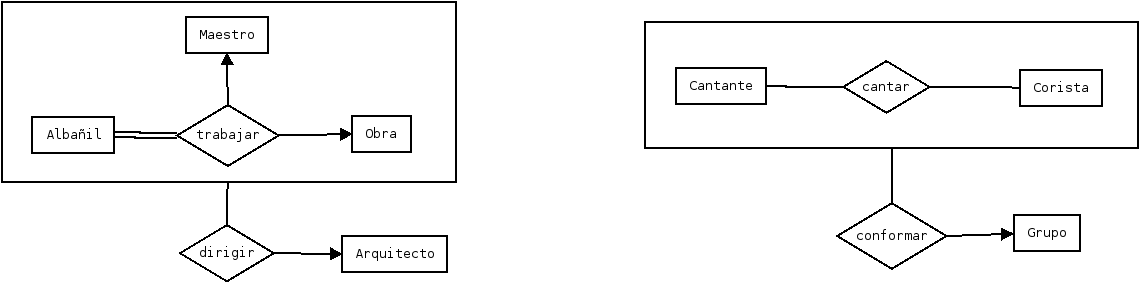
\includegraphics[scale=0.4]{agregacion.png}

            \item[iv.] Diseña una base de datos que represente los conceptos
                      revisados para crear un \textbf{diagrama E/R} (no 
                      consideres el modelo E/R extendido) \vspace{.2cm}

                      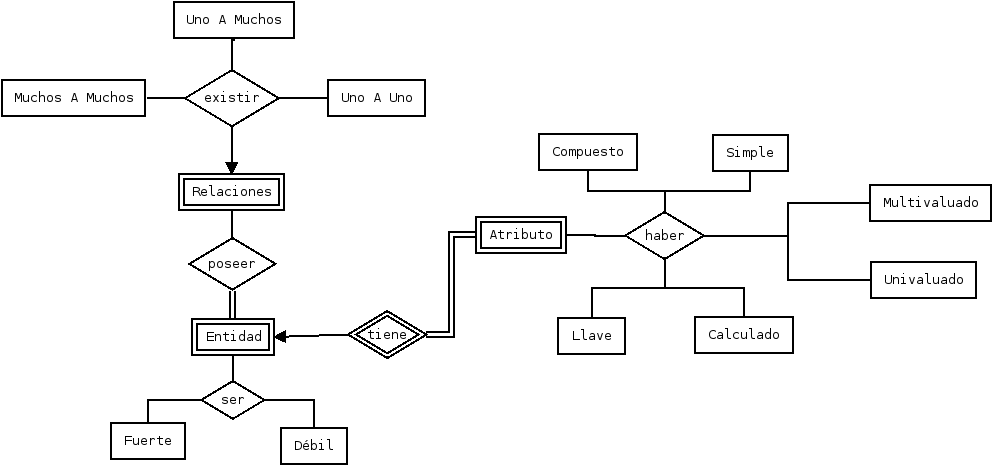
\includegraphics[scale=0.4]{modelo_eR.png}

        \end{itemize}

    \section{Modelo Entidad/Relación}

        \subsection*{a. Empresa de envíos}

        Una \textbf{empresa de envíos} desea modernizar su administración
        de envíos, para lo cual se desea diseñar una \textbf{base de datos}
        a partir de las siguientes restricciones del negocio:
        
            \begin{itemize}
                \item[i.] La empresa cuenta con una serie de \textbf{vehículos para 
                        transporte}, de los cuales se desea almacenar su
                        \textbf{número de motor, marca, modelo, tipo, descripción, 
                        fecha de compra y precio de compra}. Cada vehículo estará
                        a cargo de un \textbf{supervisor} para la realización de 
                        su mantenimiento. Todo transporte debe tener asignado un
                        sólo supervisor y cada supervisor estará a cargo de al
                        menos un vehículo.
                \item[ii.] Los vehículos son de \textbf{tres tipos: motos, van y 
                        aviones}. De las \textbf{motos} interesa almacenar su
                        \textbf{cilindraje}, de los \textbf{van} su 
                        \textbf{capacidad} y de los \textbf{aviones} el tipo
                        de \textbf{fuselaje}. De los \textbf{supervisores} 
                        interesa conocer el \textbf{RFC, nombre completo, 
                        dirección, teléfono} y \textbf{transportes a su cargo}.
                \item[iii.] La empresa maneja \textbf{dos tamaños básicos} para las
                            mercancías: \textbf{sobres y paquetes}. De los 
                            \textbf{sobres} interesa conocer el \textbf{peso} y de
                            los \textbf{paquetes} las \textbf{dimensiones}. En los
                            envíos, los \textbf{sobres se asignan a una moto} para
                            su transporte y no puede haber sobres sin asignar a 
                            motos; una moto puede tener asignados varios sobres o
                            ninguno. Si la mercancía en un \textbf{paquete}, se 
                            \textbf{asignará una van} con las mismas restricciones
                            que se tienen los sobres y las motos.
                \item[iv.] De las \textbf{mercancías enviadas} se almacenará el 
                        \textbf{código, la descripción, el precio de envío, 
                        si están aseguradas} y si son \textbf{al interior de 
                        la república}. Si las mercancías son al \textbf{interior
                        de la república}, entonces se les \textbf{asignará
                        adicionalmente un avión}. No puede haber mercancías que
                        se envíen al interior de la república que no tengan
                        asignado avión. Un avión puede tener asignadas varias o 
                        ninguna mercancía de larga distancia. Una mercancía de
                        larga distancia debe tener asignada su correspondiente
                        moto o van para llevarla empresa/aeropuerto/destino final.
                \item[v.] Los \textbf{clientes} de la empresa de envíos son empresas
                        o particulares, de estos clientes interesa almacenar el
                        \textbf{código de cliente, la fecha y el total facturado}
                        a dicho cliente. Si el \textbf{cliente es un particular}
                        se almacenará su \textbf{RFC, nombre completo, dirección
                        y teléfonos}. Si el cliente es una \textbf{empresa}, se
                        almacenará el \textbf{RFC, razón social, dirección, 
                        teléfonos y correo electrónico}. 
                \item[vi.] De los \textbf{envíos de mercancías} hay que almacenar el \textbf{cliente 
                        que realiza el envío, el destinatario, la mercancía 
                        enviada y la fecha de envío}. Los clientes pueden encargar 
                        el envío de sus mercancías a dos tipos de destinatarios: 
                        \textbf{empresas o particulares}. Si el envío es a una empresa 
                        se debe enviar al menos una mercancía. Si el envío tiene 
                        como destino un particular, se cobrará el almacenaje que 
                        consiste en el 4\% del precio original del envío. En 
                        cualquiera de los dos casos se cobrará un 1\% más por 
                        cada vez que no se ha conseguido realizar la entrega. Interesa,
                        entonces almacenar el número de intentos de entrega de una 
                        mercancía a un particular y se deben almacenar todos los 
                        envíos encargados por el cliente.    
            \end{itemize}


            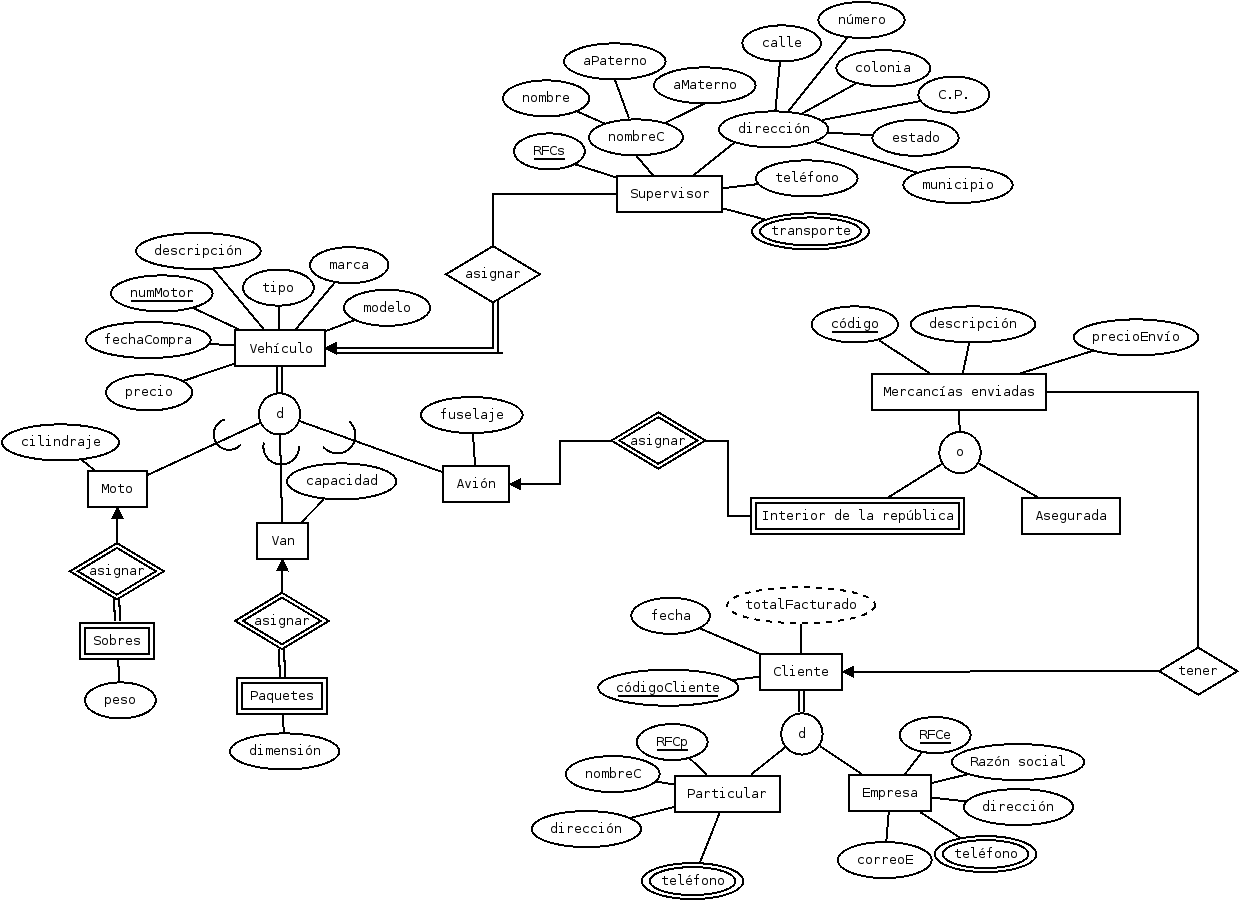
\includegraphics[scale=0.4]{empresa_envios.png}

        \subsection*{b. Sistema de información geográfica}

        La \textbf{Secretaría del Medio Ambiente y Recursos Naturales (SEMARNAT)} desea 
        crear un \textbf{SIG} (Sistema de Información Geográfica) para acceso público a 
        través de Internet. El sistema ofrecerá la siguiente información:

            \begin{itemize}
                \item Datos referentes a \textbf{ríos, afluentes, sistemas montañosos, 
                      montañas y municipios} donde se localizan.
                \item De los \textbf{ríos} se almacenará un identificador del río, nombre,
                      descripción y longitud total. Para cada río, además, se 
                      almacenarán los municipios que atraviesa la longitud del 
                      tramo del río para cada municipio bañado.
                \item De los \textbf{municipios} se almacenará un identificador para el
                      municipio, nombre y número de habitantes.
                \item Los \textbf{ríos} pueden ser afluentes de otros ríos, si es 
                      el caso, se desea conocer a cuál río alimentan y el municipio 
                      en el que se unen al río del que son afluentes.
                \item En cuanto a los \textbf{sistemas montañosos}, se almacenará 
                      un código, el nombre, la orientación (norte, sur, este, 
                      oeste), la longitud, la altura máxima y los municipios 
                      que ocupa. Los sistemas están formados por \textbf{montañas} 
                      de los que se almacena un código, un nombre, descripción y
                      altura. Se debe considerar que una montaña sólo pertenecerá
                      a un sistema montañoso. Se requiere también almacenar también 
                      el municipio o municipios en los que se encuentra, ya que 
                      hay casos en los que una montaña es compartida por varios
                      municipios.
                \item Las \textbf{montañas} además pueden tener un \textbf{origen} 
                      volcánico o de \textbf{plegamiento}. En el caso de que
                      su origen sea volcánico, se desea almacenar el tipo de 
                      volcán y si es de plegamiento, se almacenará el periodo 
                      geológico de dicho plegamiento.
                \item \textbf{Algunos ríos y montañas} son elementos geológicos 
                      \textbf{monitoreados por satélite}. De dichos elementos 
                      se desea almacenar la fecha en la que se comienzan a 
                      monitorear y el satélite que realiza el seguimiento. 
                      Un satélite puede monitorear varios elementos. De los 
                      satélites se desea almacenar su identificador, nombre 
                      y descripción.
            \end{itemize}

            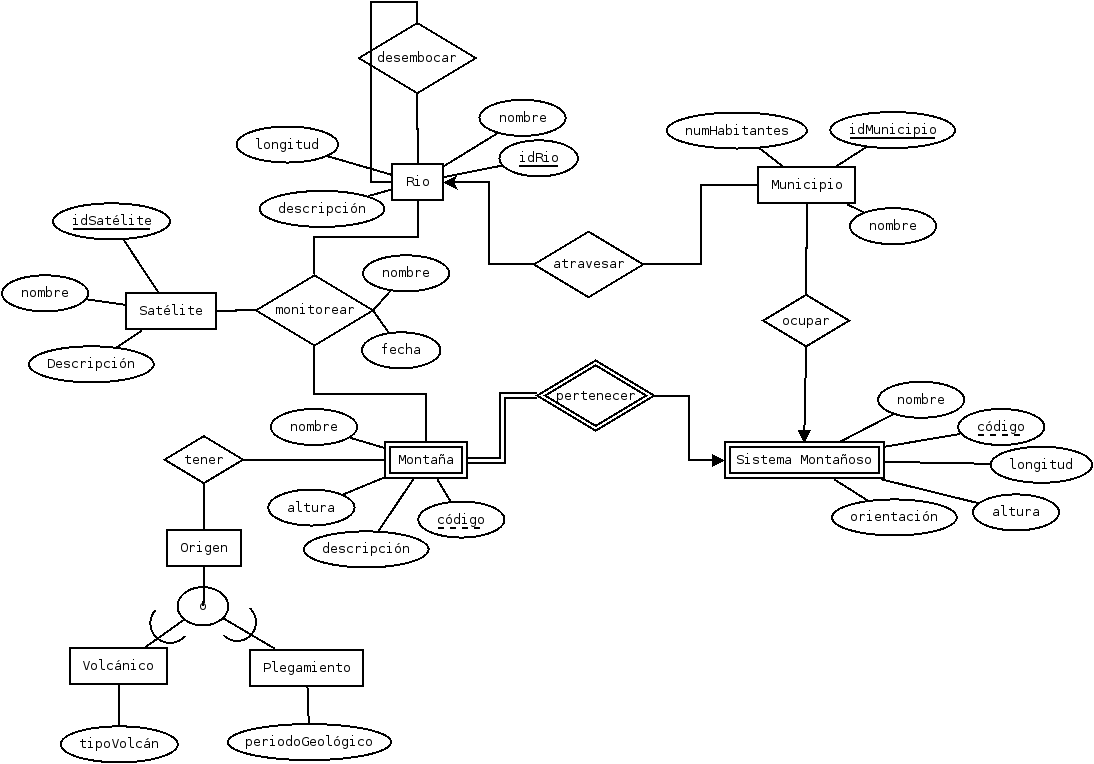
\includegraphics[scale=0.4]{sistema_infog.png}

    \section{Ingeniería inversa}

    Una \textbf{compañía celular} requiere una base de datos para realizar un 
    seguimiento de sus \textbf{clientes, sus planes de suscripción y los 
    teléfonos móviles} que están utilizando. El \textbf{diagrama E/R} de la 
    siguiente figura muestra entidades de interés para la compañía y las 
    relaciones entre ellas. Tomando como base el esquema proporcionado, 
    responde a las siguientes preguntas justificando tu respuesta. Para cada 
    pregunta, identificar el o los elementos en el diagrama E/R que utilizaste 
    para tu respuesta. En caso de que alguna pregunta no se cumpla en el 
    diagrama actual, indica las modificaciones que deberían hacerse para que 
    se permita dicho comportamiento. 

    \begin{itemize}
          \item ¿Un cliente puede tener un número ilimitado de planes?
          \item ¿Un cliente puede existir sin un plan?
          \item ¿Es posible crear un plan sin saber quién es el cliente?
          \item ¿El operador quiere limitar los tipos de dispositivos que se 
                pueden vincular a un tipo de plan específico?
          \item ¿Es posible mantener los datos relativos a un teléfono sin 
                conectarlo a un plan?
          \item ¿Puede un teléfono puede asociar a varios planes?
          \item Supongamos que existe un tipo de teléfono que puede utilizar múltiples sistemas operativos.
          \item[] ¿Esta situación podría tener cabida dentro del modelo incluido en la figura?
          \item ¿La empresa capaz de realizar un seguimiento de un fabricante sin mantener información sobre
                  sus teléfonos?
          \item ¿Puede el mismo sistema operativo puede utilizar en múltiples tipos de dispositivos?
          \item Hay dos relaciones entre el Cliente y el Plan. Explicar en qué difieren.
          \item Caracterizar el grado y la cardinalidad de la relación que une al cliente a sí mismo. Explicar su
                  significado.
          \item ¿Es posible vincular un teléfono a un cliente específico en un plan con múltiples clientes?
          \item ¿Puede la compañía rastrear un teléfono sin identificar su sistema operativo?
    \end{itemize}

\end{document}